%%%%%%%%%%%%%%%%%%%%%%%%%%%%%%%%%%%%%%%%%%%
%
% From a template maintained at https://github.com/jamesrobertlloyd/cbl-tikz-poster
%
% Code near the top should be fairly standard and not need to be changed
%  - except for the document class
% Code lower down is more likely to be customised
%
%%%%%%%%%%%%%%%%%%%%%%%%%%%%%%%%%%%%%%%%%%%

%%%%%%%%%%%%%%%%%%%%%%%%%%%%%%%%%%%%%%%%%%%
%
% Document class
%
% Change this if you want a different size / orientation poster etc
%
%%%%%%%%%%%%%%%%%%%%%%%%%%%%%%%%%%%%%%%%%%%

\documentclass[landscape,a0b,final,a4resizeable]{a0poster}
%\documentclass[portrait,a0b,final,a4resizeable]{a0poster}


\usepackage{multicol}
\usepackage{color}
\usepackage{shadow}
\usepackage{morefloats}
\usepackage{cite}
\usepackage[pdftex]{graphicx}
\usepackage{rotating}
\usepackage{amsmath, amsthm, amssymb, bm}
\usepackage{array}
\usepackage{nth}
\usepackage[square,numbers]{natbib}
\usepackage{booktabs}
%\usepackage{xcolor}

%%%%%%%%%%%%%%%%%%%%%%%%%%%%%%%%%%%%%%%%%%%
%
% TIKZ packages and common definitions
%
% Add extra things as per your tikz needs
%
%%%%%%%%%%%%%%%%%%%%%%%%%%%%%%%%%%%%%%%%%%%

\usepackage{../common/picins}
\usepackage{tikz}
\usetikzlibrary{shapes.geometric,arrows,chains,matrix,positioning,scopes,calc}
\tikzstyle{mybox} = [draw=white, rectangle]

%%%%%%%%%%%%%%%%%%%%%%%%%%%%%%%%%%%%%%%%%%%
%
% myfig
%
% \myfig - replacement for \figure
% necessary, since in multicol-environment 
% \figure won't work        
%                 
%%%%%%%%%%%%%%%%%%%%%%%%%%%%%%%%%%%%%%%%%%%

\newcommand{\myfig}[3][0]{
\begin{center}
  \vspace{1.5cm}
  \includegraphics[width=#3\hsize,angle=#1]{#2}
  \nobreak\medskip
\end{center}}

%%%%%%%%%%%%%%%%%%%%%%%%%%%%%%%%%%%%%%%%%%%
%
% mycaption                
%
% \mycaption - replacement for \caption
% necessary, since in multicol-environment \figure and
% therefore \caption won't work
%
%%%%%%%%%%%%%%%%%%%%%%%%%%%%%%%%%%%%%%%%%%%

%\newcounter{figure}
\setcounter{figure}{1}
\newcommand{\mycaption}[1]{
  \vspace{0.5cm}
  \begin{quote}
    {{\sc Figure} \arabic{figure}: #1}
  \end{quote}
  \vspace{1cm}
  \stepcounter{figure}
}

%%%%%%%%%%%%%%%%%%%%%%%%%%%%%%%%%%%%%%%%%%%
%
% Some standard colours
%
%%%%%%%%%%%%%%%%%%%%%%%%%%%%%%%%%%%%%%%%%%%

\definecolor{camlightblue}{rgb}{0.601 , 0.8, 1}
\definecolor{camdarkblue}{rgb}{0, 0.203, 0.402}
\definecolor{camred}{rgb}{1, 0.203, 0}
\definecolor{camyellow}{rgb}{1, 0.8, 0}
\definecolor{lightblue}{rgb}{0, 0, 0.80}
\definecolor{white}{rgb}{1, 1, 1}
\definecolor{whiteblue}{rgb}{0.80, 0.80, 1}

%%%%%%%%%%%%%%%%%%%%%%%%%%%%%%%%%%%%%%%%%%%
%
% Some look and feel definitions
%
%%%%%%%%%%%%%%%%%%%%%%%%%%%%%%%%%%%%%%%%%%%

\setlength{\columnsep}{0.03\textwidth}
\setlength{\columnseprule}{0.0018\textwidth}
\setlength{\parindent}{0.0cm}

%%%%%%%%%%%%%%%%%%%%%%%%%%%%%%%%%%%%%%%%%%%
%
% \mysection - replacement for \section*
% 
% Puts a pretty box around some text
% TODO - any other thoughts for what this box should look like
%
%%%%%%%%%%%%%%%%%%%%%%%%%%%%%%%%%%%%%%%%%%%

\tikzstyle{mysection} = [rectangle, 
									draw=none, 
									shade, 
									outer color=camlightblue!30,
									inner color=camlightblue!30,
									text width=0.965\columnwidth,
									text centered,
									rounded corners=20pt,
									minimum height=0.11\columnwidth]

\newcommand{\mysection}[1]
{
\begin{center}
  \begin{tikzpicture}
    \node[mysection] {\sffamily\bfseries\LARGE#1};
  \end{tikzpicture}
\end{center}
}

%%%%%%%%%%%%%%%%%%%%%%%%%%%%%%%%%%%%%%%%%%%
%
% Set the font
%
% TODO - Not sure what a canonical choice is - feel free to modify
%
%%%%%%%%%%%%%%%%%%%%%%%%%%%%%%%%%%%%%%%%%%%

\renewcommand{\familydefault}{cmss}
\sffamily

%%%%%%%%%%%%%%%%%%%%%%%%%%%%%%%%%%%%%%%%%%%
%
% Poster environment
%
% Centres everything and can be used to define the width of the content
%
%%%%%%%%%%%%%%%%%%%%%%%%%%%%%%%%%%%%%%%%%%%

\newenvironment{poster}{
  \begin{center}
  \begin{minipage}[c]{0.96\textwidth}
}{
  \end{minipage} 
  \end{center}
}

%%%%%%%%%%%%%%%%%%%%%%%%%%%%%%%%%%%%%%%%%%%
%
% This is probably a good place to put content specific packages and definitions
%
%%%%%%%%%%%%%%%%%%%%%%%%%%%%%%%%%%%%%%%%%%%

%\usepackage{preamble}
\usepackage{tabularx}

\def\newarrow{\mbox{\begin{tikzpicture}
             \useasboundingbox{(-3pt,-4.5pt) rectangle (19pt,1pt)};
             \draw[->] (0,-0.07)--(17pt,-0.07);\end{tikzpicture}}}
             
\usepackage[autostyle]{csquotes}  

%%%%%%%%%%%%%%%%%%%%%%%%%%%%%%%%%%%%%%%%%%%
%
% The document environment starts here
%
%%%%%%%%%%%%%%%%%%%%%%%%%%%%%%%%%%%%%%%%%%%

\begin{document}

%%%%%%%%%%%%%%%%%%%%%%%%%%%%%%%%%%%%%%%%%%%
%
% Begin the poster environment - centres things and potentially changes the width
%
%%%%%%%%%%%%%%%%%%%%%%%%%%%%%%%%%%%%%%%%%%%

\begin{poster}

%%%%%%%%%%%%%%%%%%%%%%%%%%%%%%%%%%%%%%%%%%%
%
% Potentially add some space at the top of the poster
%
%%%%%%%%%%%%%%%%%%%%%%%%%%%%%%%%%%%%%%%%%%%

\vspace{0\baselineskip}

%%%%%%%%%%%%%%%%%%%%%%%%%%%%%%%%%%%%%%%%%%%
%
% Draw the header as a TIKZ picture
%
% Using TIKZ to allow for easy alignment
%
%%%%%%%%%%%%%%%%%%%%%%%%%%%%%%%%%%%%%%%%%%%

\begin{center}
\begin{tikzpicture}[x=0.5\textwidth]
    % Dummy nodes at edges for spacing
    % TODO - a better way?
    \node at (+1, 0) {};    
    \node at (-1, 0) {};
    % Set the size of the badges
    \def \badgeheight {0.08\textwidth}
    % Title text
    \node[inner sep=0,text width=0.7\textwidth,text centered,font=\Huge] (Title) at (0,0) 
    {
      {\sffamily \Huge \textbf{Statistical Model criticism using Kernel Two Sample Tests}}\\
      {\huge\sffamily James Robert Lloyd and Zoubin Ghahramani}\\
      \vspace{-0.3\baselineskip}
      {\large\sffamily Department of Engineering, University of Cambridge, UK}
    };
    % Cambridge badge
    \node [mybox] (Cambridge Badge) at (-0.9, 0) {
        \includegraphics[height=\badgeheight]{../badges/cam-crest-and-text.pdf}
    };
    % CBL badge
    \node [mybox] (CBL Badge) at (+0.9, 0) {
        
\includegraphics[height=\badgeheight]{../badges/cbl-badge-cropped.png}
    };
    % MIT badge
    %\node [mybox] (MIT Badge) at (+0.825, 0) {
    %    
\includegraphics[height=\badgeheight]{../badges/MIT2.jpg}
    %};
    % QR code
    %\node [mybox] (QR code) at (-0.95, 0) {
    %    
\includegraphics[height=\badgeheight]{../badges/QR.png}
    %};
\end{tikzpicture}
\end{center}

%%%%%%%%%%%%%%%%%%%%%%%%%%%%%%%%%%%%%%%%%%%
%
% Spacing between title and main body
%
%%%%%%%%%%%%%%%%%%%%%%%%%%%%%%%%%%%%%%%%%%%

\vspace{1\baselineskip}

%%%%%%%%%%%%%%%%%%%%%%%%%%%%%%%%%%%%%%%%%%%
%
% Columns environment
%
%%%%%%%%%%%%%%%%%%%%%%%%%%%%%%%%%%%%%%%%%%%

\begin{multicols}{3}

%%%%%%%%%%%%%%%%%%%%%%%%%%%%%%%%%%%%%%%%%%%
%
% Start of content
%
%%%%%%%%%%%%%%%%%%%%%%%%%%%%%%%%%%%%%%%%%%%

\large

\mysection{Summary of paper}

\vspace{1\baselineskip}

\begin{itemize}
  \item We think that model criticism is very important but underrepresented in much of the machine learning literature
  \vspace{0.5\baselineskip}
  \item We investigated the application of a kernel hypothesis test to model criticism and give examples of its usage
  \vspace{0.5\baselineskip}
  \item But most importantly we would like more people to be mindful of the benefits of model criticism
\end{itemize}

\vspace{1\baselineskip}

\mysection{What is model criticism?}

\vspace{1\baselineskip}

\vspace{1\baselineskip}

\newpage

\mysection{Why do we need model criticism?}

\vspace{1\baselineskip}

\begin{quotation}
``A man in daily muddy contact with field experiments could not be expected to have much faith in any direct assumption of independently distributed normal errors''
\end{quotation}

\vspace{1\baselineskip}

But perhaps more importantly, vigorous criticism is an essential part of the scientific method

%\item \dots and that can lead to false conclusions\dots

%\begin{quotation}
%``We were seeing things that were 25-standard deviation moves, several 
%days in a row'
%\end{quotation}

\begin{center}
  \large
  \tikzstyle{block} = [rectangle, draw, fill=blue!20, 
                       text width=0.2\columnwidth, text centered, rounded corners, minimum height=3em]
  \tikzstyle{line} = [draw, -latex', line width=10pt]
  \tikzstyle{thin line} = [draw, -latex', line width=5pt]
  \tikzstyle{cloud} = [draw, ellipse,fill=red!20,minimum height=2em]
    
  \begin{tikzpicture}[node distance = 0.3\columnwidth]
    % Place nodes
    \node [block] at (0, 0) (hypothesis) {Hypothesis generation};
    \node [block] at (0.4\columnwidth, 0) (infer) {Deduction and inference};
    %\node [cloud] at (0.4\columnwidth, -0.2\columnwidth) (apply) {Application};
    %\node [cloud] at (0.4\columnwidth, +0.2\columnwidth) (data) {Data};
    \node [block] at (0.8\columnwidth, 0) (criticise) {Evaluation and \bf{criticism}};
    % Draw edges
    \path [line] (hypothesis.east) -- (infer.west);
    \path [line] (infer.east) -- (criticise.west);
    %\path [thin line] (infer.south) -- (apply.north);
    %\path [thin line] (data.south) -- (infer.north);
    %\path [thin line] (data.south east) -- (criticise.north west);
    %\path [thin line] (hypothesis.north east) -- (data.south west);
    %\path [thin line] (criticise.south west) -- (apply.north east);
    \draw[->, , line width=10pt] (criticise.south) .. controls (0.6\columnwidth,-0.2\columnwidth) and (0.2\columnwidth,-0.2\columnwidth) .. (hypothesis.south);
  \end{tikzpicture}
\end{center}

%\vspace{1\baselineskip}

Machine learning has been focused on model performance i.e.\ validation, which provides little information on \emph{how to improve} a model

\vspace{1\baselineskip}

\mysection{Kernel two sample tests}

\vspace{1\baselineskip}

\vspace{1\baselineskip}

\newpage

\mysection{What do neural networks dream about?}

\vspace{1\baselineskip}

We trained RBMs to generate MNIST digits.
We then used kernel two sample tests to show us digits underrepresented (left) and overrepresented (right) by the model.

\begin{center}
  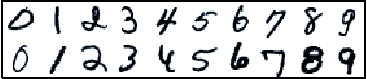
\includegraphics[width=0.48\columnwidth]{../figures/many_rbm_cond_witness_peaks}
  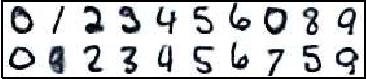
\includegraphics[width=0.48\columnwidth]{../figures/many_rbm_cond_witness_troughs}
\end{center}

Aside from some mistakes, the overrepresented digits appear fuzzy.
But maybe we just need to go deeper and use a DBN?

\begin{center}
  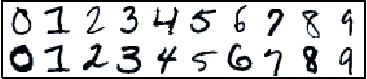
\includegraphics[width=0.48\columnwidth]{../figures/dbn_ft_cond_witness_peaks}
  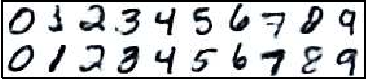
\includegraphics[width=0.48\columnwidth]{../figures/dbn_ft_cond_witness_troughs}
\end{center}

Here the overrepresented digits appear to have entire sections faded out.
The extra layers do not appear to have removed the fuzziness, it has just become more correlated.

Note well, these overrepresented digits are not outliers, they are digits that are consistently produced by the models.

\vspace{1\baselineskip}

\mysection{Other examples}

\vspace{1\baselineskip}

\vspace{1\baselineskip}

\mysection{Discussion}

\vspace{1\baselineskip}

\vspace{1\baselineskip}

\end{multicols}

\end{poster}

\end{document}

